%%%%%%%%%%%%%%%%%%%%%%%%%%%%%%%%%%%%%%%%%%%%%%%%
\begin{frame}
	\frametitle{}
	\Background[1] 
	\begin{center}
	{ {\Huge 第五章~~贝塞尔函数 (8学时)}}
	\end{center}    
\end{frame}
%%%%%%%%%%%%%%%%%%%%%%%%%%%%%%%%%%%%%%%%%%%%%

\section{1.贝塞尔方程}

\begin{frame}
	\frametitle{方程的建立}
	\begin{exampleblock} {例1、建立贝塞尔方程}
		对于半径为$r_0$的侧面绝缘的薄均匀圆盘,边界温度始终保持为0度,当盘的初始温度已知时 ($\Psi(x,y)$),求体系的温度分布函数。
    \end{exampleblock}
	\begin{center}
		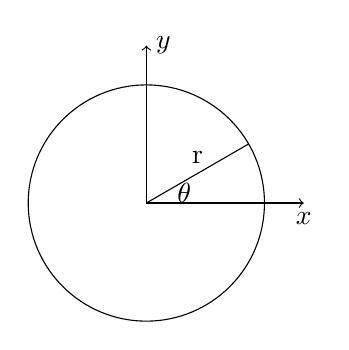
\begin{tikzpicture}
			\def\k{2};
			\node (O) at (0, 0) {};
			\node (A) at (0,1.5) {};
			\node (B) at (30:1.5) {} ;	
			\draw [ ->] (0,0) --  (\k,0)  node[below] {$x$};
			\draw [ ->]  (0,0) -- ( 0,\k)   node[right] {$y$};
			\draw  (0,0) -- (30:1.5) node[midway,above] {r};
			\draw (0,0) circle (1.5cm);
			\path (0,0) ++(15: .5) node{$\theta$};
		\end{tikzpicture}
	\end{center}
\end{frame}	

\begin{frame}
	\alert{ 解:}	这是一个温度场,是非稳恒场,服从热传导方程:\\
	$\begin{cases}
		u_t=a^2 [u_{xx}   +u_{yy}] ~~~~ (0< x^2 +y^2 <r_0 ^2, t>0)\\
		u(x,y,t)|_{x^2+y^2=r_0 ^2}= 0 \\
		u(x,y,t)|_{t=0}= \Psi(x,y)
	\end{cases} $\\	\vspace{0.6em}
	考虑到圆域边界条件,得使用极坐标描述\\
\end{frame}

\begin{frame}
	\frametitle{}
	试证明极坐标拉普拉斯算子为:
	\[[u_{xx}   +u_{yy}]= [ {	\frac{\partial^2 u }{\partial r^2 } +\frac{1}{r } \frac{\partial u }{\partial r } +
	\frac{1}{r^2 } \frac{\partial ^2 u }{\partial \theta ^2
	} }]\]
	\证 ~基本变换关系为 
\[ \begin{cases}
	 x=r\cos \theta\\
	 y=r\sin \theta
	\end{cases}\]
对于函数 $ u(x,y)=u(r\cos \theta,r\sin \theta)$ 计算导数:
\[
\begin{aligned}
	\frac{\partial u}{\partial r}&=\frac{\partial u}{\partial x } \frac{\partial x}{\partial r }+  \frac{\partial u}{\partial y } \frac{\partial y}{\partial r } = \cos \theta \frac{\partial u}{\partial x } +  \sin \theta \frac{\partial u}{\partial y } \\
	\frac{\partial u}{\partial \theta}&=\frac{\partial u}{\partial x } \frac{\partial u}{\partial \theta }+  \frac{\partial u}{\partial y } \frac{\partial y}{\partial \theta } = -r \sin \theta \frac{\partial u}{\partial x } +  r\cos \theta \frac{\partial u}{\partial y } \\
\end{aligned}\]
\end{frame}

\begin{frame}
	改写成矩阵形式:
	\[ 
\begin{aligned}
	&\begin{bmatrix}
	   \frac{\partial u}{\partial r} \\
	   \frac{\partial u}{\partial \theta} 
	\end{bmatrix}
	=
	\begin{bmatrix}
		\cos \theta &  \sin \theta \\
		-r \sin \theta& r\cos \theta \\  
	\end{bmatrix}
	\begin{bmatrix}
		\frac{\partial u}{\partial x} \\
		\frac{\partial u}{\partial y} 
	 \end{bmatrix}\\
	&\begin{bmatrix}
		\frac{\partial u}{\partial r} \\
		\frac{\partial u}{\partial \theta} 
	 \end{bmatrix}
	 =
	 \begin{bmatrix}
		1 &  0 \\
		0 & r \\  
	\end{bmatrix}
	 \begin{bmatrix}
		 \cos \theta &  \sin \theta \\
		 -\sin \theta& \cos \theta \\  
	 \end{bmatrix}
	 \begin{bmatrix}
		 \frac{\partial u}{\partial x} \\
		 \frac{\partial u}{\partial y} 
	  \end{bmatrix}\\
	 &\begin{bmatrix}
		\frac{\partial u}{\partial x} \\
		\frac{\partial u}{\partial y} 
	 \end{bmatrix}
	 =
	 \begin{bmatrix}
		 \cos \theta &  -\sin \theta \\
		 \sin \theta& \cos \theta \\  
	 \end{bmatrix}
	 \begin{bmatrix}
		1 &  0 \\
		0 & 1/r \\  
	\end{bmatrix}
	 \begin{bmatrix}
		 \frac{\partial u}{\partial r} \\
		 \frac{\partial u}{\partial \theta} 
	  \end{bmatrix}\\
\end{aligned}
	  \]
\end{frame}


\begin{frame}
	\frametitle{}
	\[ 
\begin{aligned}
	 &\begin{bmatrix}
		\frac{\partial u}{\partial x} \\
		\frac{\partial u}{\partial y} 
	 \end{bmatrix}
	 =
	 \begin{bmatrix}
		 \cos \theta &  -\sin \theta \\
		 \sin \theta& \cos \theta \\  
	 \end{bmatrix}
	 \begin{bmatrix}
		 \frac{\partial u}{\partial r} \\
		\frac{1}{r} \frac{\partial u}{\partial \theta} 
	  \end{bmatrix}\\
	&\begin{bmatrix}
		\frac{\partial u}{\partial x} \\
		\frac{\partial u}{\partial y} 
	 \end{bmatrix}
	 =
	 \begin{bmatrix}
		 \vec{e}_r & \vec{e}_\theta 
	 \end{bmatrix}
	 \begin{bmatrix}
		 \frac{\partial u}{\partial r} \\
		\frac{1}{r} \frac{\partial u}{\partial \theta} 
	  \end{bmatrix} \\
	&\nabla= \vec{e}_r \frac{\partial }{\partial r} +   \vec{e}_\theta \frac{1}{r} \frac{\partial }{\partial \theta} \\
	&\begin{aligned}
		\nabla ^2 &=\nabla \cdot \nabla \\
		&= (\vec{e}_r \frac{\partial }{\partial r} +   \vec{e}_\theta  \frac{1}{r}\frac{\partial }{\partial \theta})\cdot (\vec{e}_r \frac{\partial }{\partial r} +   \vec{e}_\theta \frac{1}{r} \frac{\partial }{\partial \theta})\\
	\end{aligned}	
\end{aligned}	
	\] 
\end{frame}

\begin{frame}
	\[ \begin{aligned}
	\nabla ^2 &= \vec{e}_r \cdot\frac{\partial }{\partial r}  (\vec{e}_r \frac{\partial }{\partial r} +   \vec{e}_\theta \frac{1}{r} \frac{\partial }{\partial \theta})+  \vec{e}_\theta \cdot \frac{1}{r} \frac{\partial }{\partial \theta} (\vec{e}_r \frac{\partial }{\partial r} +   \vec{e}_\theta \frac{1}{r} \frac{\partial }{\partial \theta})\\
	&=\vec{e}_r \cdot (\frac{\partial \vec{e}_r}{\partial r} \frac{\partial }{\partial r} + \vec{e}_r \frac{\partial ^2 }{\partial r ^2}+  \frac{\partial \vec{e}_\theta}{\partial r} \frac{1}{r}\frac{\partial }{\partial \theta}+  \vec{e}_\theta\frac{\partial }{\partial r} (\frac{1}{r}\frac{\partial }{\partial \theta})) \\
	&\hspace{1em} + \vec{e}_\theta \cdot (\frac{1}{r}\frac{\partial \vec{e}_r}{\partial \theta} \frac{\partial }{\partial r} + \vec{e}_r \frac{1}{r} \frac{\partial }{\partial \theta} \frac{\partial }{\partial r} + \frac{1}{r} \frac{\partial  \vec{e}_\theta}{\partial \theta} \frac{1}{r} \frac{\partial }{\partial \theta} + \vec{e}_\theta \frac{1}{r} \frac{\partial }{\partial \theta} (\frac{1}{r} \frac{\partial }{\partial \theta} )
	) \\
	&=\vec{e}_r \cdot (0 \frac{\partial }{\partial r} + \vec{e}_r \frac{\partial ^2 }{\partial r ^2}+  0\frac{\partial }{\partial \theta}+  \vec{e}_\theta\frac{\partial }{\partial r} (\frac{1}{r}\frac{\partial }{\partial \theta})) \\
	&\hspace{1em} + \vec{e}_\theta \cdot (\vec{e}_\theta \frac{1}{r}\frac{\partial }{\partial r} + \vec{e}_r \frac{1}{r} \frac{\partial }{\partial \theta} \frac{\partial }{\partial r} + \frac{1}{r} (-\vec{e}_r) \frac{1}{r} \frac{\partial }{\partial \theta} + \vec{e}_\theta \frac{1}{r^2} \frac{\partial ^2 }{\partial \theta ^2}
	) \\
	&=  \frac{\partial^2  }{\partial r^2 } +\frac{1}{r } \frac{\partial  }{\partial r } +\frac{1}{r^2 } \frac{\partial ^2  }{\partial \theta ^2} 
	\end{aligned}\] 
~\\ \vspace{1em}
\alert{\textit{Tips:\hspace{1em}}} $\frac{\partial  \vec{e}_\theta}{\partial \theta}=-\vec{e}_r ;\quad \frac{\partial  \vec{e}_\theta}{\partial r}=0 ;  \quad \frac{\partial  \vec{e}_r}{\partial r}=0 ; \quad\frac{\partial  \vec{e}_r}{\partial \theta}=\vec{e}_\theta $ 
\end{frame}

\begin{frame}
	\frametitle{极坐标系下的方程}
	$\begin{cases}
		\displaystyle	u_t=a^2 [ {	\frac{\partial^2 u }{\partial r^2 } +\frac{1}{r } \frac{\partial u }{\partial r } +
		\frac{1}{r^2 } \frac{\partial ^2 u }{\partial \theta ^2
		} }], ~~~~ (0<r<r_0, t>0)\\
		u(r_0,\theta)=0,~~~~~~~~~~~~ 0<\theta <2\pi 	\\
		u(r,\theta,t =0)=\Psi(r,\theta) ,~~~~~~~~~~~~ 0<\theta <2\pi 	
	\end{cases} $\\
	令:$u(r,\theta,t) =R(r)\Theta(\theta)T(t)$,  代回原方程,得:
	\begin{equation*}
		R\Theta T'=a^2 [ R'' \Theta T + \dfrac{1}{r} R' \Theta T  + \dfrac{1}{r^2} R \Theta '' T(t)  ]
	\end{equation*}
	整理:
	\begin{equation*}
		\frac{T'}{a^2T} =\frac{R''}{R}+\frac{1}{r} \frac{R'}{R} +\frac{1}{r^2} \frac{\Theta ''} {\Theta}  =-\lambda
	\end{equation*}
	转化为两个方程:
	\begin{equation*}
		T'(t)+\lambda a^2T(t)=0  ~~~~~....... ~~~~~~(1)
	\end{equation*}	
	方程1是衰减模型,已求解!\\
\end{frame}	

\begin{frame}
	\begin{equation*}
		r^2 \frac{R'' (r)}{R(r)}+r \frac{R'(r)}{R(r)} + \lambda r^2 +\frac{\Theta ''(\theta)} {\Theta (\theta)} =0  ~~~~~~......~~(2)
	\end{equation*}
	方程2是固有值问题,可继续分离变量:	
	\begin{equation*}
		r^2 \frac{R'' (r)}{R(r)}+r \frac{R'(r)}{R(r)} + \lambda r^2 =-\frac{\Theta ''(\theta)} {\Theta (\theta)} =\mu  
	\end{equation*}
	角向固有值问题:
	$ \begin{cases}
		\Theta ''(\theta)+\mu \Theta (\theta) =0 \\
		\Theta (\theta) =	\Theta (\theta+2\pi)  \\
		\Theta' (\theta) =	\Theta' (\theta+2\pi)  
	\end{cases} $\\	
	径向固有值问题:
	$ \begin{cases}
		r^2 R'' (r)+r R'(r) +( \lambda r^2 -\mu)R(r)=0  \\
		R(r_0)=0
	\end{cases} $\\	
\end{frame}	

\begin{frame}
	角向固有值问题有解,\\
	固有值:
	\begin{equation*}
		\mu=n^2, ~~~~~(n=0,1,2,3...)
	\end{equation*}
	固有函数:
	\begin{equation*}
		\Theta_n(\theta) = a_n \cos(n\theta)+b_n \sin(n\theta), ~~~~~(n=0,1,2,3...)
	\end{equation*}
	\begin{equation*}
		\Theta_n(\theta) = \frac{1}{\sqrt{2\pi}} e^{-i n \theta }, ~~~~~(n=0,1,2,3...)
	\end{equation*}
	~\\
	把$\mu=n^2$,代回径向方程,得径向固有值问题:\vspace{0.6em}
	\[ \boxed{ \begin{cases}
		r^2 R'' (r)+r R'(r) +( \lambda r^2 -n^2)R(r)=0  \\
		R(r_0)=0
	\end{cases} }\]	
	称为贝塞尔方程	
\end{frame}	

\begin{frame}
	\begin{exampleblock} {例2、试证明圆域波动方程的径向固有值问题也是贝塞尔方程:}~ ~
	\end{exampleblock}
	\证~圆域波动方程如下:\\
	$\begin{cases}
		u_{tt}=a^2 [u_{xx}   +u_{yy}] ~~~~ (0< x^2 +y^2 <r_0 ^2, t>0)\\
		u(x,y,t)|_{x^2+y^2=r_0 ^2}= 0 \\
		u(x,y,t)|_{t=0}= \Psi(x,y) \\
		u_t (x,y,t)|_{t=0}= \varphi  (x,y) 
	\end{cases} $\\	\vspace{0.6em}
	考察方程,发现当使用极坐标拉普拉斯算子后,整个的分离变量过得与热传导方程高度一致,(*P115)\\
	其固有值问题也是贝塞尔方程!\\ \vspace{0.6em}
	$\begin{cases}
		r^2 R'' (r)+r R'(r) +( \lambda r^2 -n^2)R(r)=0  \\
		R(r_0)=0
	\end{cases} $\\		
\end{frame}	

\begin{frame}
	\frametitle{结论: }
	贝塞尔方程是圆域极坐标条件下的一个普适的径向本征方程! \\ \vspace{2em}
	\[\begin{cases}
		r^2 R'' (r)+r R'(r) +( \lambda r^2 -n^2)R(r)=0  \\
		R(r_0)=0
	\end{cases}  \]\\	
\end{frame}	

\begin{frame}	
	在正式求解之前,先预处理一下\\
	令:
	\begin{equation*}
		x=\sqrt{\lambda} r, ~~~~y(x)= R(r) =R(\frac{x}{\sqrt{\lambda}})
	\end{equation*}
	有: 
	\[
	\begin{aligned}
		&\frac{dy}{dx} = \frac{dR}{dr} \frac{dr}{dx} = \frac{1}{ \sqrt{\lambda}} \frac{dR}{dr}\\
		&\frac{d^2y}{dx^2} = \frac{1}{\lambda} \frac{dR^2}{dr^2}\\
	\end{aligned}	
	\]
	代回原方程,
\end{frame}	

\begin{frame}
	得:
	\begin{equation*}
		\boxed{x^2\frac{d^2y}{dx^2} + x\frac{dy}{dx} +(x^2 -n^2)y=0}
	\end{equation*}
	称为n整数阶贝塞尔方程.\\ \vspace{1em}
	{\Bullet}与欧拉方程比较:
	\begin{equation*}
		x^2\frac{d^2y}{dx^2} + x\frac{dy}{dx} +n^2y=0
	\end{equation*}
	欧拉方程是一个变系数微分方程,可通过变量代换(令$t=\ln x $) 转化为常系数微分方程
	\[ \frac{d^2y}{dt^2} - n^2y=0 \]
\end{frame}	

\begin{frame}
	若同样令$t=\ln x $, 贝塞尔方程转化为 
	\[ \frac{d^2y}{dt^2} +(x^2-n^2)y=0 \]
	依然是变系数微分方程,无法进一步进行求解.\\
	因此,贝塞尔方程没有通常意义的初等函数表达式解!
\end{frame}	

\begin{frame}
	\frametitle{方程的求解}
	\begin{exampleblock} {例2、求解贝塞尔方程}
		\begin{equation*}
			x^2\frac{d^2y}{dx^2} + x\frac{dy}{dx} +( x^2 -n^2)y=0
		\end{equation*}	
	\end{exampleblock}
	\alert{ 解:}~没有通常意义的初等函数表达式解,即没有通常意义的级数解,\\
	尝试,设方程有如下非一般意义的级数解:
	\begin{equation*}
		y=\sum\limits_{k=0}^{\infty} a_k x^{s+k},  \qquad (a_0 \not =0)
	\end{equation*}	
\end{frame}	

\begin{frame}
	求导:
	\begin{equation*}
		y'=\sum\limits_{k=0}^{\infty} (s+k) a_k x^{s+k-1}
	\end{equation*}	
	\begin{equation*}
		y''=\sum\limits_{k=0}^{\infty} (s+k) (s+k-1) a_k x^{s+k-2}
	\end{equation*}	
	代回原方程(注意脚标的变化),得:
	\begin{equation*}
		\sum\limits_{k=0}^{\infty} [(s+k) ^2 -n^2]  a_k x^{s+k} + \sum\limits_{k=2}^{\infty}  a_{k-2} x^{s+k} =0
	\end{equation*}	
	第一项(k=0)系数应为零:
	\begin{equation*}
		(s+k) ^2 -n^2=0,~~ \to s_1=-n, \qquad s_2=n. 
	\end{equation*}	
\end{frame}	

\begin{frame}
	第二项(k=1)系数应为零:
	\begin{equation*}
		[(s+k) ^2 -n^2] a_1=0,\qquad \to a_1=0. 
	\end{equation*}	
	后面各项系数都为零:
	\begin{equation*}
		[(s+k) ^2 -n^2] a_k+ a_{k-2}=0, ~~~ (k=2,3,4,...)
	\end{equation*}	
	存在递推关系:
	\begin{equation*}
		a_k=-\frac{1}{(s+k) ^2 -n^2 } a_{k-2}
	\end{equation*}	
	由$a_1=0$,可推出奇数项为零 \[a_{2m+1}=0\]
	现取$s=n$, (-n 不影响解题过程),得:
	\begin{equation*}
		a_{2m}=\frac{-1}{(n+2m) ^2 -n^2 } a_{2m-2} =\frac{-1}{2m (2n+2m) } a_{2m-2}, \qquad (m=1,2,3,...)
	\end{equation*}	
\end{frame}	

\begin{frame}
	归纳,得:
	\begin{equation*}
		a_{2m}=(-1)^m  \frac{1}{2^{2m} m! (n+m) (n+m-1)... (n+1) } a_0 
	\end{equation*}	
	取:$a_0=1/2^n n!$, 得:
	\begin{equation*}
		a_{2m}=(-1)^m  \frac{1}{2^{2m+n} m! (n+m) ! }
	\end{equation*}	
	贝塞尔方程有级数特解:
	\begin{equation*}
		y(x) = \sum\limits_{m=0}^{\infty} a_{2m} x^{n+2m} 
	\end{equation*}	
	分析收敛性,发现:
	\begin{equation*}
		\lim\limits_{m\to \infty}|\frac{ a_{2m+2}} {a_{2m}}|= \lim\limits_{m\to \infty}\frac{ 1}{4(m+1)(n+m+1)} =0
	\end{equation*}	
	说明此级数必为某函数的展开式,称之为贝塞尔函数。
\end{frame}	

\begin{frame}
	记为: \[\boxed{J_n(x) = \sum\limits_{m=0}^{\infty} a_{2m} x^{n+2m}} 
		 \]
	称为n整数阶贝塞尔函数! 
\end{frame}	

\begin{frame}
	\centering
	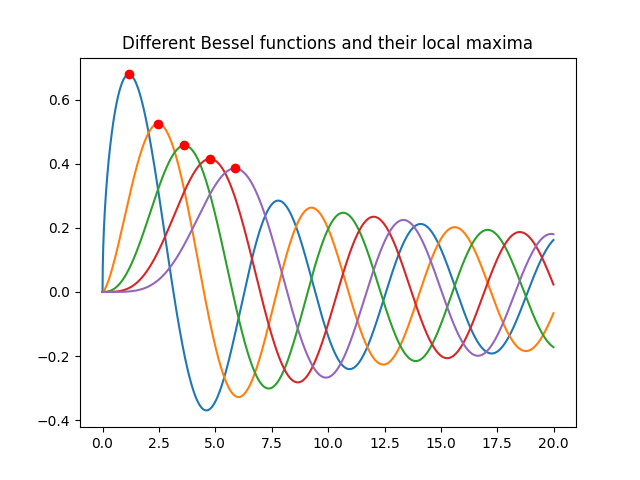
\includegraphics[width=0.8\textwidth]{figs/bessel.png}
\end{frame}	

\begin{frame}
	\begin{center}
			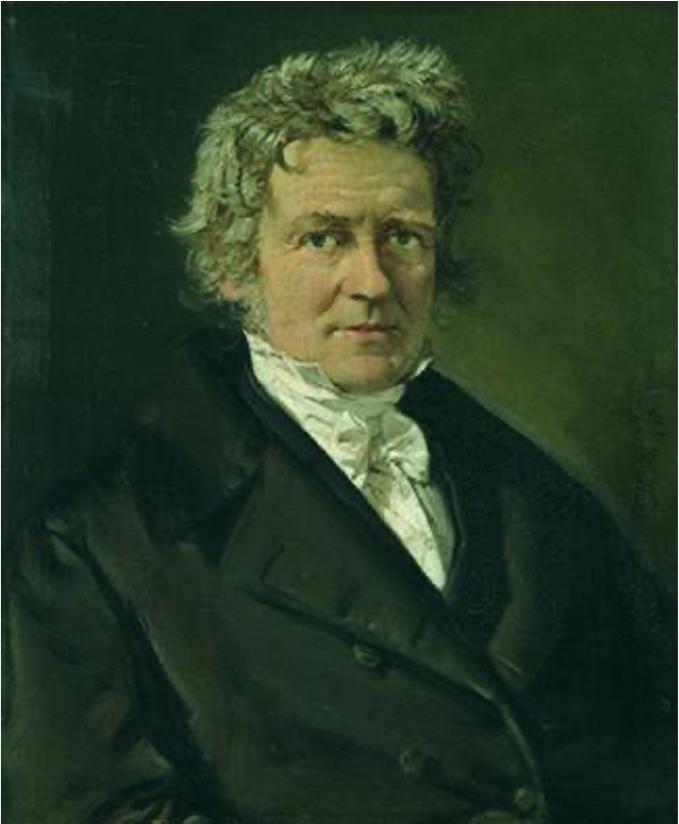
\includegraphics[width=4.2cm]{figs/fig1-3-6.png}	
	\end{center}
	贝塞尔(Bessel,Friedrich Wilhelm,1784~1846)德国天文学家,数学家,天体测量学的奠基人.
	提出贝塞尔函数,讨论该函数的一系列性质及其求值方法,为解决物理学、天文学和信息学有关问题提供了重要工具。
\end{frame}

\begin{frame}
	\frametitle{作业}
	1、由圆域波动方程导出贝塞尔方程\\
	2、求衰减模型
	\begin{equation*}
		T'(t)+\lambda a^2T(t)=0  
	\end{equation*}
	3、求角向固有值及归一化的固有函数:\\
	\[ \begin{cases}
		\Theta ''(\theta)+\mu \Theta (\theta) =0 \\
		\Theta (\theta) =	\Theta (\theta+2\pi)  \\
		\Theta' (\theta) =	\Theta' (\theta+2\pi)  
	\end{cases}  \]	
	4、求欧拉方程
\end{frame}	

\section{2.贝塞尔函数与Gamma函数}

\begin{frame}
	\frametitle{贝塞尔函数}
	零阶贝塞尔函数:
	\begin{equation*}
		J_0(x) = \sum\limits_{m=0}^{\infty} (-1)^m  \frac{1}{m! m! } (\frac{x}{2})^{2m} 
	\end{equation*}	
	n阶贝塞尔函数:
	\begin{equation*}
		J_n(x) = \sum\limits_{m=0}^{\infty} (-1)^m  \frac{1}{m! (n+m) ! } (\frac{x}{2})^{n+2m} 
	\end{equation*}	
	第二类贝塞尔函数:
	\begin{equation*}
		Y_{\alpha}(x)=\frac{J_{\alpha}(x) \cos (\alpha \pi)-J_{-\alpha}(x)}{\sin (\alpha \pi)}
	\end{equation*}	
	贝塞尔函数在除$x=0$点外的整个实数轴上收敛。
\end{frame}	

\begin{frame}
	\frametitle{$\Gamma$函数}
	为进一步讨论贝塞尔函数的性质,先讨论Gamma函数.\\  
	\begin{enumerate}
		\Item 1728年,哥德巴赫在考虑数列插值的问题, 比如我们可以计算2!,3!,是否可以计算2.5!呢? 
		\Item 他写信请教尼古拉斯·伯努利和他的弟弟丹尼尔·伯努利, 欧拉当时正好与丹尼尔·伯努利在一块,他因此得知了这个问题
		\Item 1729 年欧拉解决了这个问题! 
	\end{enumerate}
	\begin{figure}
		\centering
		\subfigure[]{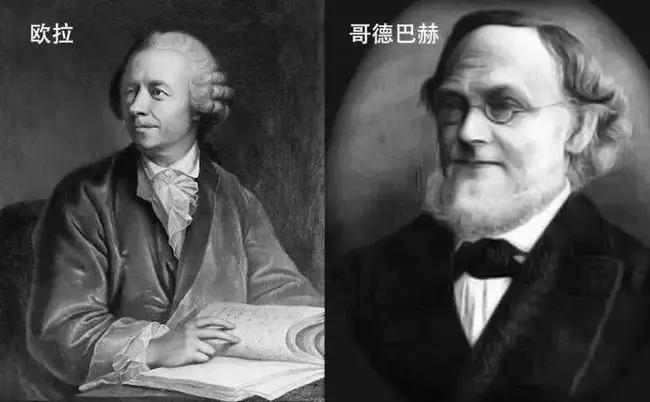
\includegraphics[width=0.45\textwidth]{figs/2022-04-02-08-43-23.png}}
	\end{figure} 
	\setcounter{subfigure}{0}
\end{frame}	

\begin{frame}
	\frametitle{$\Gamma$函数的定义}	
	\begin{equation*}
		\Gamma(x)=\int_{0}^{\infty} t^{x-1} e^{-t} dt, \qquad (x>0)
	\end{equation*}	
	
	Euler创造的$\Gamma$函数,将积分和阶乘联系在起来\\ \vspace{0.6em}
	\例 [1.试证明]
	{ \[
		\Gamma(1)=1
	   \]}
	\证 ~	
\[ \begin{aligned}
	\Gamma(1)&=\int_{0}^{\infty} t^{1-1} e^{-t} dt \\	
			&=\int_{0}^{\infty}  e^{-t} dt =1	
\end{aligned}\]
\end{frame}	

\begin{frame}	
	\frametitle{~$\Gamma$函数的性质}
	\alert{性质1:} ~试证明Gamma函数有如下递推式:
		\[\Gamma(x+1)=x \Gamma(x),\qquad (x>0)\]
	\alert{证明:}  
	\begin{equation*}
	\begin{split}
		\Gamma(x+1)&= \int_{0}^{\infty} t^{x+1-1} e^{-t} dt \\
		&= -t^x e^{-t} |_0 ^\infty + x \int_{0}^{\infty} t^{x-1} e^{-t} dt \\
		&= x \int_{0}^{\infty} t^{x-1} e^{-t} dt \\
		&=x \Gamma(x)
	\end{split}
	\end{equation*}	
\end{frame}	

\begin{frame}
	 推论: 
	\begin{equation*}
		\Gamma(x+n)=(x+n-1)(x+n-2)\cdots (x+1)x\Gamma(x)
	\end{equation*}	 
\end{frame}	

\begin{frame}
	\alert{性质2:}~试证明自变量为正整数的Gamma函数与阶乘有如下关系:
	\begin{equation*}
		\Gamma(n+1)=n!
	\end{equation*}	
	\alert{证明1:}  由递推公式
	\begin{equation*}
	\begin{split}
		\Gamma(x+1)&=x \Gamma(x) \\
		\Gamma(n+1)&=n \Gamma(n) \\
		&=n(n-1)\cdots 1 \Gamma(1) \\
		&=n! \int_{0}^{\infty}  e^{-t} dt \\
		&=n!
	\end{split}
	\end{equation*}	
\end{frame}	

\begin{frame}
	\alert{证明2:}  	 在推论中:取$x=1$
	\begin{equation*}
	\begin{split}	
		\Gamma(x+n)&=(x+n-1)(x+n-2)\cdots (x+1)x\Gamma(x)\\
		\Gamma(1+n)&=(1+n-1)(1+n-2)\cdots (1+1)1\Gamma(1)\\
		\Gamma(n+1)&=n!
	\end{split}
	\end{equation*}	 
	~~\\ \vspace{4em}
\alert{\textit{Tips:\hspace{1em}}} ~ 阶乘只是$\Gamma(x)$函数的特例!$(x=1,2,3,\cdots)$对应$ (0!, 1!, 2!,\cdots)$
\end{frame}	


\begin{frame}
	\alert{性质3:} 试证明半正整数$\Gamma$函数有如下性质 
	\begin{equation*}
		\begin{split}
		\Gamma(\frac{1}{2}) &=\sqrt{\pi} \\ 
		\qquad  \Gamma(n+\frac{1}{2}) &= \frac{(2n-1)!!}{2^n} \sqrt{\pi}
		\end{split}	
	\end{equation*}	
	\alert{证明:}  (1) 由Gamma函数定义
	\[
	\begin{aligned}
		 \Gamma(x)&=\int_{0}^{\infty} t^{x-1} e^{-t} dt, \qquad (x>0) \\
		 \Gamma(\frac{1}{2})&=\int_{0}^{\infty} t^{\frac{1}{2}-1} e^{-t} dt\\
		 &=\int_{0}^{\infty} \frac{1}{\sqrt{t}} e^{-t} dt\\
	\end{aligned}	
	\]
\end{frame}

\begin{frame}
	  \frametitle{}
	  令$x=\sqrt{t}$
	  \[
		\begin{aligned}
			 \Gamma(\frac{1}{2})
			 &=2\int_{0}^{\infty} e^{-x^2} dx\\
			 &=2\sqrt{\iint_{0}^{\infty} e^{-x^2} e^{-y^2} dxdy}\\
			 &=2\sqrt{\int_{0}^{\frac{\pi}{2}} \int_{0}^{\infty}  e^{-r^2} r dr d\theta}\\
			 &=2\sqrt{\frac{\pi}{2} \int_{0}^{\infty} r e^{-r^2} dr }\\
			 &=2\sqrt{\frac{\pi}{2}[-\frac{1}{2} e^{-r^2}]_{0}^{\infty} }\\
			 &=\sqrt{\pi}
		\end{aligned}	
		\]  
	* x,y皆取正数,是第一象限!			
\end{frame}	

\begin{frame}
	  \frametitle{}
	  (2) 由递推公式 $\Gamma(1+x)=x \Gamma(x) ,\qquad (x>0)$\\
	  \[
	\begin{aligned}
		\Gamma(1+\frac{1}{2})&= \frac{1}{2} \Gamma(\frac{1}{2}) =\frac{1}{2} \sqrt{\pi}\\
		\Gamma(2+\frac{1}{2})&= \Gamma(1+\frac{3}{2})=\frac{3}{2} \Gamma(1+\frac{1}{2}) = \frac{3}{2}\frac{1}{2}\sqrt{\pi}\\
		\Gamma(3+\frac{1}{2})& = \frac{5}{2} \frac{3}{2}\frac{1}{2}\sqrt{\pi}\\
		\Gamma(n+\frac{1}{2})& = \frac{(2n-1)!!}{2^n}\sqrt{\pi}\\
		 & = \frac{(2n)!}{2^{2n} n!}\sqrt{\pi}
	\end{aligned} 
	  \]
	证毕!
\end{frame}

\begin{frame}
	\alert{性质4:} 试证明半正整数的阶乘为
	\[(\frac{1}{2})! =  \frac{\sqrt{\pi}}{2}\]
	\[ (m-\frac{1}{2})! =\frac{(2m)!}{2^{2m} m!}\sqrt{\pi} \]
	\alert{证明:} 把如下公式从正整数向正实数延拓!
	\[\Gamma(n+1)=n!\qquad \to \qquad \Gamma(x+1)=x!, (x>0)\]
	(1) 取:$x=m-\frac{1}{2}, \qquad (m=1,2,3, \cdots )$
	\[ \begin{aligned}
		(m-\frac{1}{2})! &= \Gamma (m-\frac{1}{2}+1) \\
						 &= \Gamma (m+\frac{1}{2}) \\
						 & = \frac{(2m)!}{2^{2m} m!}\sqrt{\pi} 
	\end{aligned} \]
\end{frame}

\begin{frame}
	(2) 在上式中取$m=1$
	\[(\frac{1}{2})! =  \frac{\sqrt{\pi}}{2} \]
	~~ \\ \vspace{1em}
* 一般分数的阶乘如何求?(余元公式,Gamma函数定义式)
\[ \Gamma(x)  \Gamma(1-x) =\frac{\pi}{\sin x \pi}, \qquad  0<x<1 \]
\[ \Gamma(\frac{1}{2}+x)  \Gamma(\frac{1}{2}-x) =\frac{\pi}{\cos x \pi}, \qquad  0<x<\frac{1}{2} \]
 * 例如,求$(\pi) !$ 
 \[ (\pi)! = \Gamma(\pi +1 ) = \int_{0}^{\infty} t^{\pi} e^{-t} dt =? \]
\end{frame}

\begin{frame}
	\alert{性质5:} 试求半负整数$\Gamma$函数的值
	\begin{equation*}
		\begin{split}
		\Gamma(-\frac{1}{2}) &=-2\sqrt{\pi} \\ 
		\Gamma(-\frac{3}{2}) &=\frac{4}{3}\sqrt{\pi}
		\end{split}	
	\end{equation*}	
	\alert{解:} (1) 把递推公式 $\Gamma(1+x)=x \Gamma(x)$ 从正实数向实数延拓! \\
	并令$x=-\dfrac{1}{2}$\\
	\[
	\begin{aligned}
		 \Gamma(-\frac{1}{2})&= -2 \Gamma(1-\frac{1}{2})\\
		 &=-2 \Gamma(\frac{1}{2})\\
		 &=-2 \sqrt{\pi}
	\end{aligned}	
	\]
\end{frame}

\begin{frame}
	  \frametitle{}
	(2) 在递推公式 $\Gamma(1+x)=x \Gamma(x)$中, 令$x=-\dfrac{3}{2}$\\
	\[
	\begin{aligned}
		 \Gamma(-\frac{3}{2})&= -\frac{2}{3} \Gamma(1-\frac{3}{2})\\
		 &=-\frac{2}{3} \Gamma(-\frac{1}{2})\\
		 &=(-\frac{2}{3})(-2 \sqrt{\pi}) \\
		 &=\frac{4}{3}\sqrt{\pi} \\
	\end{aligned}	
	\] 
\end{frame}

\begin{frame}
	* 从正实数$x>0$向实数延拓 $x \in \mathbb{R} $, 导致严重的问题, 比如: 
	\[ n! =(n-1)(n-2)(n-3)\cdots 1\]
	\[ (-1)! =(-1)(-2)(-3)\cdots -\infty ? \] 
	\[\Gamma(0)= (-1)! \quad ? , \qquad \Gamma(-1)=?, \cdots\] 
	\alert{性质6:} ~试证明Gamma函数在非正整数点的极限为无穷大
	\begin{equation*}
		\lim\limits_{x\to -n }\Gamma(x)=\infty, \qquad (n=0,1,2, \cdots)
	\end{equation*}	
		\[ \frac{1}{\Gamma(-n)} =0, \qquad (n=0,1,2, \cdots) \]
\end{frame}		
\begin{frame}
\alert{证明:}  由递推公式
	\begin{equation*}
	\begin{split}
		\Gamma(x)&=\frac{1}{x} \Gamma(x+1) \\
		\lim\limits_{x\to 0 }	\Gamma(x)&=	\lim\limits_{x\to 0 } \frac{1}{x} \Gamma(x+1) =\infty \\
		\lim\limits_{x\to -1 }	\Gamma(x)&=\lim\limits_{x\to -1 } \frac{1}{x} \Gamma(x+1) =  \lim\limits_{x\to 0 } \frac{1}{x-1} \Gamma(x) =\infty \\
		& \cdots \cdots	\\	
		\lim\limits_{x\to -n }	\Gamma(x)&=\lim\limits_{x\to -n } \frac{1}{x} \Gamma(x+1) = \lim\limits_{x\to -(n-1) } \frac{1}{x-1} \Gamma(x) =\infty  
	\end{split}
	\end{equation*}	
	证毕! \\ \vspace{1em}
\alert{\textit{Tips:\hspace{1em}}} \\ 
延拓到实数域后, $\Gamma$函数存在奇点$x = 0,-1,-2,\cdots$,如果进一步延拓到复数域, 这些奇点依然存在.它们是$\Gamma$函数的一阶极点!
\end{frame}	

\begin{frame}
	\frametitle{实数域Gamma函数}
  \begin{center}
	   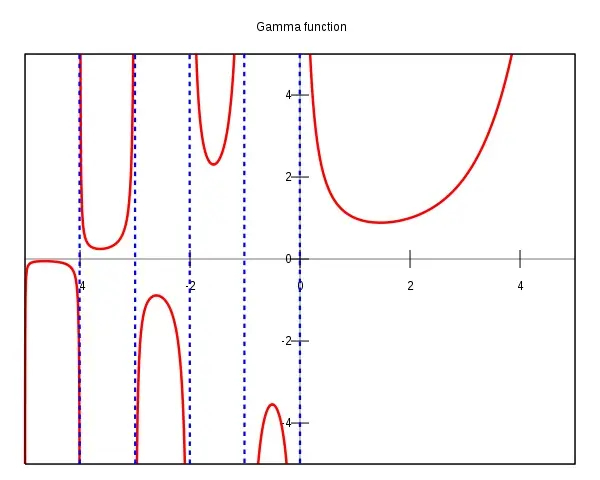
\includegraphics[width=0.85\textwidth,height=2.9in]{figs/2022-04-03-09-17-41.png}
  \end{center}
\end{frame}

\begin{frame}
	\frametitle{复数域Gamma函数}
  \begin{center}
	   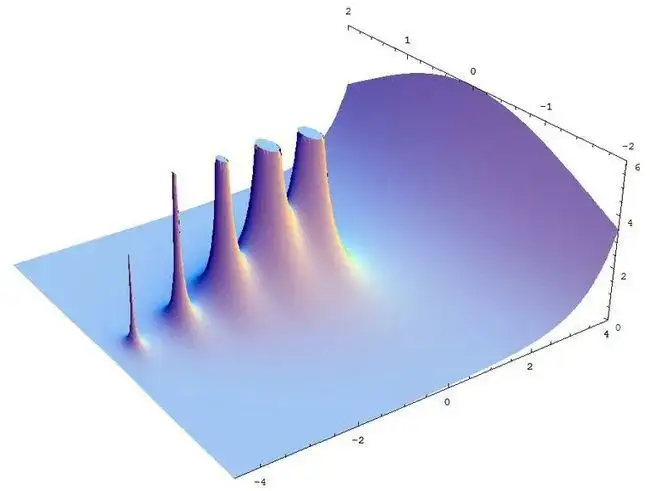
\includegraphics[width=0.85\textwidth,height=2.5in]{figs/2022-03-26-17-20-10.png}
  \end{center}
  网络教学资源, \href{https://www.bilibili.com/video/av892512155/}{点这里}
\end{frame}

\begin{frame}
	\frametitle{Gamma 函数的应用实例}
	\例 [1. 计算如下积分]{
	\[ (1)~\int_{0}^{\infty} x^2 e^{-x^2} dx, \qquad (2)~\int_{0}^{\infty} x^2 e^{-\frac{1}{2}x^2} dx \]}
	\解 ~ 比较(1)式与Gamma函数的定义式的结构,
	\[\Gamma(x)=\int_{0}^{\infty} t^{x-1} e^{-t} dt, \qquad (x>0)\]
	\[\begin{aligned}
		\int_{0}^{\infty} x^2 e^{-x^2} dx &= \int_{0}^{\infty} x^2 e^{-(x^2)} \frac{1}{2x}d(x^2)\\
		&= \frac{1}{2}\int_{0}^{\infty} (x^2)^{\frac{1}{2}} e^{-(x^2)} d(x^2)\\	
		&= \frac{1}{2}\int_{0}^{\infty} t^{\frac{3}{2}-1} e^{-t} d(t)
	\end{aligned} \]
\end{frame}

\begin{frame}
	  \frametitle{}
	  \[\begin{aligned}	
		&= \frac{1}{2}\Gamma(\frac{3}{2})  \\ 
		&= \frac{1}{2} \Gamma(1+\frac{1}{2}) \\
		&= \frac{1}{2} (\frac{1}{2})!	\\
		&= \frac{\sqrt{\pi}}{4}
	\end{aligned} \]
\end{frame}

%%%%%%%%%%%%%%%%%%%%%%%%%%%%%%%%%%%%%%%%%%%%%%%%%%%%%%%%%%%%%%%%%%%
\begin{frame}
	\frametitle{课外作业}
	\begin{enumerate}
		\item 求 $0!, \qquad \int_{0}^{\infty} x^2 e^{-\frac{1}{2}x^2} dx $
		\item 试证明 $ \frac{1}{\Gamma(-n)} =0, \qquad (n=0,1,2, \cdots) $
		\item 试证明半正整数$\Gamma$函数值的一般性公式
		\[ (m-\frac{1}{2})! =\frac{(2m)!}{2^{2m} m!}\sqrt{\pi} \qquad (m=1,2,3,\cdots) \]
		\item 试求出半负整数$\Gamma$函数值的一般性公式
		\[\Gamma(m-\frac{1}{2})=?, \qquad (m=0,-1,-2,-3,\cdots)\]	
	\end{enumerate}
\end{frame}
%%%%%%%%%%%%%%%%%%%%%%%%%%%%%%%%%%%%%%%%%%%%%%%%%%%%%%%%%%%%%%%%%%%

\section{3.贝塞尔函数的性质}

\begin{frame}
	现在讨论贝塞尔函数的性质:\\
	\alert{性质1:} 负数阶贝塞尔函数与正数阶贝塞尔函数有如下关系
	\begin{equation*}
		J_{-n}(x)=(-1)^n J_n(x)
	\end{equation*}	
	\alert{证明:}  
	用$\Gamma$ 函数重写出贝塞尔函数:
	\begin{equation*}
		J_n(x) = \sum\limits_{m=0}^{\infty} (-1)^m  \frac{1}{m! (n+m) ! } (\frac{x}{2})^{n+2m} 
	\end{equation*}	
	\begin{equation*}
		J_n(x) = \sum\limits_{m=0}^{\infty} (-1)^m  \frac{1}{m! \Gamma(n+m+1) } (\frac{x}{2})^{n+2m} 
	\end{equation*}	
	负数阶塞尔函数可写成
	\begin{equation*}
		J_{(-n)}(x) = \sum\limits_{m=0}^{\infty} (-1)^m  \frac{1}{m! \Gamma(-n+m+1) } (\frac{x}{2})^{-n+2m} 
	\end{equation*}	
\end{frame}	

\begin{frame}
	对于 $m<n$ 的项,分母中的Gamma函数为无穷大,因此都为零,要去除:
	\begin{equation*}
		J_{(-n)}(x) = \sum\limits_{m=n}^{\infty} (-1)^m  \frac{1}{m! \Gamma(-n+m+1) } (\frac{x}{2})^{-n+2m} 
	\end{equation*}	
	令 $m-n=k$, 有 $m=n+k $, 
	\begin{equation*}
		J_{(-n)}(x) = (-1)^n\sum\limits_{k=0}^{\infty} (-1)^k  \frac{1}{(n+k)! \Gamma(k+1) } (\frac{x}{2})^{n+2k} 
	\end{equation*}	
	\begin{equation*}
		J_{-n} (x) = (-1)^n\sum\limits_{k=0}^{\infty} (-1)^k  \frac{1}{(n+k)! k! } (\frac{x}{2})^{n+2k} =(-1)^n J_{n} (x)
	\end{equation*}	
	证毕!
\end{frame}	

\begin{frame}
	\alert{性质2:} 半整数阶贝塞尔函数与三角函数有如下关系
	\begin{equation*}
		J_{1/2} (x) =\sqrt{\frac{2}{\pi x}} \sin x,  \qquad  J_{-1/2} (x) =\sqrt{\frac{2}{\pi x}} \cos x
	\end{equation*}	
	\alert{证明:}  基于Gamma函数,可以写出半整数阶贝塞尔函数
	\begin{equation*}
		J_n(x) = \sum\limits_{m=0}^{\infty} (-1)^m  \frac{1}{m! \Gamma(n+m+1) } (\frac{x}{2})^{n+2m} 
	\end{equation*}	
	\begin{equation*}
		J_{1/2}(x) = \sum\limits_{m=0}^{\infty} (-1)^m  \frac{1}{m! \Gamma(1/2+m+1) } (\frac{x}{2})^{1/2+2m} 
	\end{equation*}	
\end{frame}	

\begin{frame}
	其中, 
	\begin{equation*}
		\begin{split}
			\Gamma(1/2+m+1) &= (\frac{2m+1}{2}) \Gamma(1/2+m) \\
			& = (\frac{2m+1}{2}\frac{2m-1}{2})  \Gamma(1/2+m-1) \\
			&\cdots \cdots \\
			& = \frac{(2m+1)!!}{2^{m+1}} \Gamma(1/2) \\
			& = \frac{(2m+1)!!}{2^{m+1}} \sqrt{\pi} \\
		\end{split}	
	\end{equation*}	
\end{frame}	

\begin{frame}
	代回,有:
	\begin{equation*}
		J_{1/2}(x) = \sqrt{\frac{2}{\pi x}} \sum\limits_{m=0}^{\infty} (-1)^m  \frac{x^{2m+1}}{(2m+1)!} 
	\end{equation*}	 
	\begin{equation*}
		J_{1/2}(x) = \sqrt{\frac{2}{\pi x}} \sin x  
	\end{equation*}	 
	同理,有 
	\begin{equation*}
		J_{-1/2}(x) = \sqrt{\frac{2}{\pi x}} \cos x  
	\end{equation*}	 
	\alert{证毕!} 
\end{frame}

\begin{frame}
	\frametitle{课堂作业}
	\begin{enumerate}
		\item 求 \[\Gamma(-\frac{1}{2}), (-\frac{1}{2}) !\]
		\item 证明: \[ J_{-1/2}(x) = \sqrt{\frac{2}{\pi x}} \cos x \]
	\end{enumerate}
\end{frame}

\begin{frame}
	\alert{性质3:} 贝塞尔函数的导数与递推式 \\
	\begin{equation*}
		\begin{split}
			\frac{d}{d x}\left[x^{n} J_{n}(x)\right]= &x^{n} J_{n-1}(x),\qquad \cdots (1) \\
			\frac{d}{d x}\left[x^{-n} J_{n}(x)\right]=& -x^{-n} J_{n+1}(x) ,\qquad \cdots (2) \\
			2 n J_{n}(x)=&xJ_{n-1}(x)+x J_{n+1}(x) ,\qquad \cdots (3) \\
			2 J_{n}^{\prime}(x)=&J_{n-1}(x)-J_{n+1}(x) ,\qquad \cdots (4) 
		\end{split}
	\end{equation*}		
	由贝塞尔函数的$\Gamma$函数形式 
	\begin{equation*}
		J_n(x) = \sum\limits_{m=0}^{\infty} (-1)^m  \frac{1}{m! \Gamma(n+m+1) } (\frac{x}{2})^{n+2m} 
	\end{equation*}	 
	\alert{证明(1)式} : 上等式两端同乘$x^n$ 再求导:
	\begin{equation*}
	\begin{split}
		\frac{d}{dx} [x^n J_n(x)]&= \frac{d}{dx}\sum\limits_{m=0}^{\infty} (-1)^m  
		\frac{1}{m! \Gamma(n+m+1) } (\frac{x^{2n+2m}}{2^{n+2m}})\\	
	\end{split}
	\end{equation*}		
\end{frame}	

\begin{frame}
	\begin{equation*}
		\begin{split}
			\frac{d}{dx} [x^n J_n(x)] &=\sum\limits_{m=0}^{\infty} (-1)^m  
			\frac{1}{m! \Gamma(n+m+1) } (\frac{(2n+2m)x^{2n-1+2m}}{2^{n+2m}})\\
			&=x^n\sum\limits_{m=0}^{\infty} (-1)^m  
			\frac{1}{m! \Gamma(n-1+m+1) } (\frac{x^{n-1+2m}}{2^{n-1+2m}})\\ 
			&=x^n J_{n-1}(x) ,\qquad \cdots (1) 
		\end{split}
	\end{equation*}	
	\alert{证明 (2)式}: 同理,得:
	\begin{equation*}
		\begin{split}
		\frac{d}{d x}\left[x^{-n} J_{n}(x)\right]&=-x^{-n} J_{n+1}(x) ,\qquad \cdots (2) \\
		\end{split}
	\end{equation*}	 
\end{frame}

\begin{frame}
	\alert{证明 (3)和(4)式}: 把(1)(2)二式左端求导
	\begin{equation*}
		\begin{split}
			\frac{d}{dx} [x^n J_n(x)] &=n x^{n-1} J_n(x) + x^n J'_n(x)=x^n J_{n-1}(x) \\
			\frac{d}{d x}\left[x^{-n} J_{n}(x)\right]&=-n x^{-n-1} J_n(x) + x^{-n} J'_n(x)= -x^{-n} J_{n+1}(x)
		\end{split}
	\end{equation*}	
两式消去$J'_n(x)$得:
	\begin{equation*}
		2 n J_{n}(x)=x J_{n-1}(x)+x J_{n+1}(x)  ,\qquad \cdots (3)
	\end{equation*}	 	
两式消去$J_n(x)$得:
	\begin{equation*}
	2 J_{n}^{\prime}(x)=J_{n-1}(x)-J_{n+1}(x)  ,\qquad \cdots (4)
	\end{equation*}	 
\alert{证毕!} 
\end{frame}

\begin{frame}
	\alert{性质4:} 证明n阶贝塞尔函数有如下零点近似公式
	\[ \mu_{m}^{n} \approx m \pi+\frac{n \pi}{2}+\frac{3 \pi}{4}\]
	\alert{解:}对n(整数)阶贝塞尔方程
	\begin{equation*}
		x^2\frac{d^2y}{dx^2} + x\frac{dy}{dx} +(x^2 -n^2)y=0
	\end{equation*}
	做变量代换 \[ y=\frac{u}{\sqrt{x}}\] 
	得到 u(x)的方程:
	\begin{equation*}
		u'' +[1+\frac{\frac{1}{4}-n^2}{x^2}] u=0
	\end{equation*}
	当$x \to \infty $ 有方程:
	\begin{equation*}
		u'' + u=0 
	\end{equation*}	
\end{frame}	

\begin{frame}
	通解为:\[u=A\cos(x+\theta)\]
	确定A和$\theta$ (不证),得n阶贝塞尔函数的渐近公式\\
	\begin{equation*}
		J_{n}(x) \approx \sqrt{\frac{2}{\pi x}} \cos \left(x-\frac{n \pi}{2}-\frac{\pi}{4}\right)
	\end{equation*}
	令$J_{n}(x)=0$,由上式可得n阶贝塞尔函数的零点近似公式:
	\begin{equation*}
		\mu_{m}^{n} \approx m \pi+\frac{n \pi}{2}+\frac{3 \pi}{4}
	\end{equation*}
\end{frame}	


\begin{frame}
	\frametitle{固有值问题}
	对于圆域热传导方程或波动方程,其径向方程为
	\[\begin{cases}
		r^2 R'' (r)+r R'(r) +( \lambda r^2 -n^2)R(r)=0  \\
		R(r_0)=0
	\end{cases}  \]
	解为n阶贝塞尔函数$R(r)=J_n(x) = J_n(\sqrt{\lambda}r)$ \\ \vspace*{2em}
	{\Bullet} 零边界条件 $R(r_0)=0$对应$J_n(\sqrt{\lambda}r_0)=0$\\ 
	因此零边界条件下的本征解, 正是贝塞尔函数的零点!
\end{frame}	

\begin{frame}
	基此确定:\\	
	(1)固有值:
	\[ \sqrt{\lambda}r_0 = \mu_{m}^{n}  \qquad \to \qquad \lambda_m ^n =(\frac{\mu_{m}^{n}}{r_0})^2 \]
	(2)固有函数:\[R_m ^n(r) = J_n (\frac{\mu_{m}^{n}}{r_0}r) \]
\end{frame}

\begin{frame}
	\frametitle{}
	\alert{性质5:} 试证明n阶贝塞尔函数有如下零点递推式
	\[ J'_n(\mu_m ^n)= - J_{n+1}(\mu_m ^n)\]
	\alert{证明:}~由微分公式(2) 
 	\begin{equation*}
	\begin{split}
	 \frac{d}{d x}\left[x^{-n} J_{n}(x)\right]=& -x^{-n} J_{n+1}(x) ,\qquad \cdots (2) \\
	 -n x^{-n-1} J_n(x) + x^{-n} J'_n(x)&= -x^{-n} J_{n+1}(x) \\
	 -n J_n(x) + x J'_n(x)&= -x J_{n+1}(x) \\
	 -n 0 + x J'_n(\mu_m ^n)&= -x J_{n+1}(\mu_m ^n) \\
	 J'_n(\mu_m ^n)&= - J_{n+1}(\mu_m ^n)
 	\end{split}
	\end{equation*}	
\end{frame}

\begin{frame}
	\alert{性质6:} 贝塞尔函数正交归一性\\
	固有函数体现塞尔函数的正交归一性:
	\begin{equation*}
		\int_0 ^{r_0} r J_n (\frac{\mu_{m} ^{n}}{r_0}r) J_n (\frac{\mu_{k} ^{n}}{r_0}r) dr =?
	\end{equation*}
	\alert{证明:}对径向方程做等价变换
	\begin{equation*}
		r^2 R''+r R' +(\lambda r^2 -n^2)R=0 
	\end{equation*}	
	\begin{equation*}
		r R''+ R' +((\frac{\mu_{m}^{n}}{r_0})^2 r -\frac{n^2}{r})R=0  
	\end{equation*}	
	\begin{equation*}
		(r R')' +((\frac{\mu_{m}^{n}}{r_0})^2 r -\frac{n^2}{r})R=0  
	\end{equation*}	
\end{frame}	

\begin{frame}
	令:\[J_n (\frac{\mu_{m}^{n}}{r_0}r)=R_1, \qquad J_n (\frac{\mu_{k}^{n}}{r_0}r) =R_2\]
	有
	\begin{equation*}
		(r R_1')' +((\frac{\mu_{m}^{n}}{r_0})^2 r -\frac{n^2}{r})R_1=0  \cdots (1)
	\end{equation*}	 
	\begin{equation*}
		(r R_2')' +((\frac{\mu_{m}^{n}}{r_0})^2 r -\frac{n^2}{r})R_2=0  \cdots (2) 
	\end{equation*}	
	$(1)\times R_2,  (2)\times R_1,$所得两次相减,并做积分,有
	\begin{equation*}	
		\int_0 ^{r_0} \left[\left(\frac{\mu_{m}^{(n)}}{r_0}\right)^{2}-\left(\frac{\mu_{k}^{(n)}}{r_0}\right)^{2}\right] r R_{1} R_{2} dr 
		=\int_0 ^{r_0}  [R_{1}\left(r R_{2}^{\prime}\right)^{\prime}-R_{2}\left(r R_{1}^{\prime}\right)^{\prime}] dr
	\end{equation*}
\end{frame}	

\begin{frame}
	\begin{equation*}
		\begin{split}
			=& [r R_1 R_2']|_0 ^{r_0} - [r R_2 R_1']|_0 ^{r_0} + \int_0 ^{r_0} r R_2' R_1 dr - \int_0 ^{r_0} rR_1' R_2 dr\\
			=& \int_0 ^{r_0} rR_2'R_1 dr - \int_0 ^{r_0} rR_1'R_2 dr\\
			=& 0
		\end{split}
	\end{equation*}	
	\begin{equation*}	
		\to \qquad	\int_0 ^{r_0} r R_{1} R_{2} dr = 0
	\end{equation*}
	正交性,\alert{证毕!}
\end{frame}	

\begin{frame}
	证明归一性:
	\begin{equation*}
		r^2 R''+r R' +(\lambda r^2 -n^2)R=0 
	\end{equation*}	
	\begin{equation*}
		2r^2 R'R''+2r (R')^2 +(\lambda r^2 -n^2)R'R=0 
	\end{equation*}	
	 整理:
	\begin{equation*}
		[r^2 (R')^2 + (\lambda r^2 -n^2)R^2]'=2 \lambda rR^2
	\end{equation*}	
\end{frame}	

\begin{frame}
	\begin{equation*}
		\begin{split}
			\int_0 ^{r_0} r R^2 dr =& \frac{1}{2\lambda} \int_0 ^{r_0} [r^2 (R')^2 + (\lambda r^2 -n^2)R^2]' dr  \\
			=& \frac{1}{2\lambda} |r^2 (R')^2 + (\lambda r^2 -n^2)R^2 |_0 ^{r_0} \\
			=& \frac{1}{2\lambda} r_0^2 (R'(r_0))^2 \\
			=& \frac{1}{2} r_0^2 [J'_n(\mu_m ^n)]^2 \\
			=& \frac{r_0^2}{2} [J_{n+1}(\mu_m ^n)]^2
		\end{split}
	\end{equation*}	
\end{frame}	


%%%%%%%%%%%%%%%%%%%%%%%%%%%%%%%%%%%%%%%%%%%%%%%%%%%%%%%%%%%%%%%%%%%
\begin{frame}
	\frametitle{课外作业}
	\begin{enumerate}
		\item 试证明
		\begin{equation*}
			\Gamma(1/2)=\sqrt{\pi}, \qquad J_{-1/2}(x) = \sqrt{\frac{2}{\pi x}} \cos x  
		\end{equation*}
		\item 试证明零点递推公式  \[ J'_n(\mu_m ^n)= - J_{n+1}(\mu_m ^n)\]
		\item 设函数$f(r)$的贝塞尔展开式为
		\begin{equation*}
			f(r)=\sum_{m=1}^\infty c_m J_n(\frac{\mu_m ^n}{r_0} r)
		\end{equation*}	
		试证明其展开系数为: 
		\begin{equation*}
			c_m=\frac{2} {r^2_0 J_{n+1} ^2 (\mu_m ^n)} \int_0 ^{r_0} f(r) J_n(\frac{\mu_m ^n}{r_0} r) r dr 
		\end{equation*}	
	\end{enumerate}
\end{frame}
%%%%%%%%%%%%%%%%%%%%%%%%%%%%%%%%%%%%%%%%%%%%%%%%%%%%%%%%%%%%%%%%%%%

\section{4.贝塞尔函数的应用}
\begin{frame}
	\frametitle{应用实例}
	求解圆域热传导问题 \\
	$\left\{
		\begin{array}{l}
		\dfrac{\partial u}{\partial t}=a^{2}\left(\dfrac{\partial^{2} u}{\partial r^{2}}+\dfrac{1}{r} 
		\dfrac{\partial u}{\partial r}+\dfrac{1}{r^{2}} \dfrac{\partial^{2} u}{\partial \theta^{2}}\right), 0<r<R, 0<\theta<2 \pi \\
		\left. u\right|_{r=R}=0,\left.u\right|_{t=0}=\varphi(r, \theta)
	\end{array}
	\right. $\\
	\alert{解:} 令 
	\begin{equation*}
		u(r,\theta,t)= T(t) V(r, \theta) 
	\end{equation*}	
	代入方程,进行第一次分离变量,得衰减方程:\[T'+\lambda a^2 T=0, \qquad \cdots (1) \]	
\end{frame}

\begin{frame}
	及亥姆霍兹方程:
	$\left\{
	\begin{array}{l}
		\frac{\partial^{2} V}{\partial r^{2}}+\frac{1}{r} \frac{\partial V}{\partial r}+\frac{1}{r^{2}} 
		\frac{\partial^{2} V}{\partial \theta^{2}}+\lambda V=0, 0<r<R, 
		0 \leq \theta \leq 2 \pi \\
		\left.V\right|_{r=R}=0, 0 \leq \theta \leq 2 \pi
		\end{array}
	\right.$\\
	令\[V(r, \theta) =F(r)G(\theta)\], 代入亥姆霍兹方程, 得两个方程\\
	\[G''+\mu G=0, \qquad \cdots (2) \]
	\[r^2 F''+r F' +(\lambda r^2 -\mu )F=0, \qquad \cdots (3) \]
\end{frame}	

\begin{frame}
	方程(1)的解为:\[T(t)=Ae^{-\lambda a^2 t}\]
	方程(2)的解为:\[G(\theta)=C_1\cos\sqrt{\mu}\theta + C_2\sin \sqrt{\mu}\theta \]
	由周期性边界条件,有$G(2\pi)=G(0)$, 必有$\cos \sqrt{\mu}\theta =1 $, 得\\
	固有值:
	\[\mu = n^2, \qquad (n=0,1,2,\cdots)\]
	固有函数:
	\[G_0(\theta)=\frac{1}{2}a_0, G_n(\theta)= a_n\cos n \theta + b_n \sin n \theta, \qquad (n=0,1,2,\cdots)\]
	固有函数也可写成 $ G_n(\theta)=a_n e^{-i n \theta} =\frac{1}{\sqrt{2\pi}} e^{-i n \theta}$
\end{frame}	

\begin{frame}
	将固有值代入方程(3),得方程 
	\[r^2 F''+r F' +(\lambda r^2 -n^2 )F=0 \]
	令 $x=\sqrt{\lambda} r, y(x)=F(x/\sqrt{\lambda})$, 
	方程转化为标准整数贝赛尔方程:
	\begin{equation*}
		x^2\frac{d^2y}{dx^2} + x\frac{dy}{dx} +(x^2 -n^2)y=0
	\end{equation*}
	则方程(3)的零边界条件解用贝赛尔函数的零点表示:\\
	固有值:
	\[\lambda_m ^n =(\frac{\mu_{m}^{n}}{R})^2 \]
	固有函数:\[F_m ^n(r) = J_n (\frac{\mu_{m}^{n}}{R}r) \]
\end{frame}	
\begin{frame}
	原方程的基本解为:
	\begin{equation*}
		u(r,\theta,t) =F_m ^n (r) G_n(\theta) e^{-\lambda_m a^2 t}
	\end{equation*}
	叠加解为:
	\begin{equation*}
		u(r,\theta,t) =\sum_{n=0}^{\infty} \sum_{m=0}^{\infty} A_m ^n F_m ^n (r) G_n(\theta) e^{-\lambda_m a^2 t}
	\end{equation*}
	应用初值条件, 
	\begin{equation*}
		\varphi(r, \theta)=\sum_{n=0}^{\infty} \sum_{m=0}^{\infty} A_m ^n F_m ^n (r) G_n(\theta) 
	\end{equation*}
	利用正交归一性确定系数$A_m ^n$
\end{frame}	

\begin{frame}
	\begin{equation*}
		\begin{split}
				 &\int_0 ^{2\pi} G_k ^* (\theta) \varphi(r, \theta) d\theta =\sum_{n=0}^{\infty} \sum_{m=0}^{\infty} A_m ^n F_m ^n (r) \int_0 ^{2\pi} G^* _k(\theta) G_n(\theta)  d\theta	\\ 
				 &\int_0 ^{2\pi} G_n  ^* (\theta) \varphi(r, \theta) d\theta = \sum_{m=0}^{\infty} A_m ^n F_m ^n (r)\\ 
				 &\int_0 ^{R} \int_0 ^{2\pi} G_n ^* (\theta) r J_n (\frac{\mu_{k}^{n}}{R}r) \varphi(r, \theta) d\theta dr = \sum_{m=0}^{\infty} A_m ^n \int_0 ^{R} r J_n (\frac{\mu_{k}^{n}}{R}r)J_n (\frac{\mu_{m}^{n}}{R}r) dr \\
				 &\int_0 ^{R} \int_0 ^{2\pi} G_n ^* (\theta) r J_n (\frac{\mu_{m}^{n}}{R}r) \varphi(r, \theta) d\theta dr = A_m ^n \frac{R^2}{2} [J_{n+1}(\mu_m ^n)]^2\\ 
				 &A_m ^n=	\frac{2}{R^2[J_{n+1}(\mu_m ^n)]^2} \int_0 ^{R} \int_0 ^{2\pi} G_n ^* (\theta) r J_n (\frac{\mu_{m}^{n}}{R}r) \varphi(r, \theta) d\theta dr 
		\end{split}
	\end{equation*}
\end{frame}	

\begin{frame}
	\frametitle{课外作业}
	1、证明 
	\begin{equation*}
		J_{3/2}(x)=\sqrt{\frac{2}{\pi x}} [\frac{1}{x}\sin x -\cos x]
	\end{equation*}
	2、证明
	\begin{equation*}
		\frac{d}{d x}\left[x^{-n} J_{n}(x)\right]=-x^{-n} J_{n+1}(x) 
	\end{equation*}	
	3、用分离变量法求解圆域热传导方程
	\[\begin{cases}
		u_t=a^2 (u_{xx}+u_{yy}), \qquad (0<r<1) \\
		u\mid_{r=1}=0 \\
		u\mid_{t=0}=\cos^2\theta
	\end{cases}\]
	4、求柱面坐标系的拉普拉斯并用分离变量法求解柱面热传导方程	
\end{frame}	

%%%%%%%%%%%%%%%%%%%%%%%%%%%%%%%%%%%%%%%%%%%%%%%%

\section{5. Dirac函数}
\subsection{定义}
\begin{frame}
	  \frametitle{引入}
	  {\Bullet}设有一条质量为$1$,长度为$2l$ 的均匀直线(段).则直线的线密度为$\rho=1/2l$\\
	  若将直线的中点放置于坐标轴的原点,则密度函数为: 
	  \[\rho(x)=\left\{\begin{array}{c}
		\frac{1}{2 l}, \qquad (-l \leq x \leq l) \\
		0, \quad (x<-l, x>l)
		\end{array}\right.\]
	 积分得质量:
	 \[\int_{-\infty}^{+\infty} \rho(x) d x= 1\]
	 显然:
	 \[\int_{a}^{b} \rho(x) d x =1, \qquad (-l,l) \subset (a,b) \]
\end{frame}

\begin{frame}
	  \frametitle{~~$\delta$函数的定义}	 
	{\Bullet} 考虑当$l \to 0$时, 线段变为质点. 质点的密度函数记为$\delta(x)$,有
	\[\delta(x)=\left\{\begin{array}{c}
		\infty, \quad(x=0) \\
		0, \quad(x \neq 0)
		\end{array}\right. \]
	\[\int_{-\infty}^{+\infty} \delta(x) d x=1 \]
	量子力学中,这么定义:
	\[\delta(x)=\left\{\begin{array}{c}
		1, \quad(x=0) \\
		0, \quad(x \neq 0)
		\end{array}\right. \]
	\[\int_{-\infty}^{+\infty} \delta(x) d x=1 \]
\end{frame}

\begin{frame}
	  \frametitle{}
	  考虑到量子化, 一般写成一个连续实函数的序列: 
	  \[\lim_{n\to\infty} \int_{-\infty}^{+\infty} \delta_n (x) d x=1 \]

	  {\Tips} 在很多问题中,我们需要用数学语言描述“点”的相关性质,这就需要推广古典函数概念,引入广义函数(a generalized function).Dirac函数是历史上第一个广义函数,也是使用最广的.
\end{frame}

\subsection{性质}
\begin{frame}
	\frametitle{$\delta$函数的性质}
	\begin{columns}
		\begin{column}[t]{0.46\linewidth}
			\[\int_{a}^{b} \delta(x) d x=1 , \quad 0\in(a,b)\]
			\[\int_{-\infty}^{+\infty} \delta(x) \psi (x) d x=\psi  (0) \]
			\[\int_{a}^{b} \delta(x) \psi (x) d x=\psi (0)  , \quad 0\in(a,b)\]
			\[ \int_{-\infty}^{+\infty} \delta(x-x_0) \psi (x) d x=\psi  (x_0) \]
		\end{column}
		\begin{column}[t]{0.46\linewidth}
	  \[ \delta(-x)=\delta(x)\]
	  \[ \delta'( -x ) = - \delta'( x ) \]
	  \[ \delta(\alpha x ) = \frac{\delta( x ) }{\left|\alpha \right|} \]
	  \[ x\delta'( x ) = - \delta( x ) \]
	  \[ x\delta_{\lambda}( x ) = \lambda \delta_{\lambda}( x ) \]
	  \[ f(x)\delta( x-a ) = f(a)\delta( x-a ) \]
	  \[ \delta( \sin x ) = \sum_{n=0}^{\infty} \delta(x-n\pi)\]
		\end{column}
	\end{columns}
\end{frame}

\begin{frame}
	  \frametitle{}
	  \例 [1. 试证明$\delta$函数是偶函数 ]
	  {\[ \delta(-x)=\delta(x)\]}
	  \证 ~  \[
		\begin{aligned}
			\int_{-\infty}^{+\infty} \delta(-x) \psi (x) d x &= \int_{+\infty}^{-\infty} \delta(x') \psi (-x') d (-x') \\
			&= \int_{-\infty}^{+\infty} \delta(x') \psi (-x') d (x') \\
			&=  \psi (-x') | _{x'=0}\\
			&=  \psi (0) \\
			&=  \int_{-\infty}^{+\infty} \delta(x) \psi (x) d x 
		\end{aligned}
		   \]
		得证!
\end{frame}

\begin{frame}
	\frametitle{}
	\例 [2. 试证明$\delta$函数的导数是奇函数  ]
	{\[ \delta'(-x) = - \delta'(x)\]}
	\证 ~  \[
	  \begin{aligned}
		\int_{-\infty}^{+\infty} \delta'(x) \psi (x) d x &= \delta(x) \psi (x)|_{-\infty}^{+\infty} - \int_{-\infty}^{+\infty} \delta(x) \psi' (x) d x \\
		  &=  - \int_{-\infty}^{+\infty} \delta(x) \psi' (x) d x \\
		  &=  - \psi' (0)
	  \end{aligned}
		 \]
\end{frame}

\begin{frame}
	  \frametitle{}
	  \[
		\begin{aligned}
		  \int_{-\infty}^{+\infty} \delta'(-x) \psi (x) d x &= \int_{+\infty}^{-\infty} \delta'(x') \psi (-x') d (-x') \\
			&= \int_{-\infty}^{+\infty} \delta'(x') \psi (-x') d (x') \\
			&=  \psi' (-x') _{x'=0}\\
			&=  \psi' (0) 
		\end{aligned}
		   \]
		评毕!\\ \vspace{1em}
		推论:\[ \int_{-\infty}^{+\infty} \delta^{(n)}(-x) \psi (x) d x = (-1)^n \psi^{(n)} (0)\]
\end{frame}

\begin{frame}
	\frametitle{}
	\例 [3. 试证明 ]
	{\[ x\delta(x)  = 0\]}
	\证 \[
		\begin{aligned}
		  \int_{-\infty}^{+\infty} x\delta(x) \psi (x) d x &= \int_{-\infty}^{+\infty} \delta(x) [x \psi (x)] d x \\
		    &=  [x \psi (x)] \mid_{x=0} \\
			&=  0\psi (0) \\
			&=  0
		\end{aligned}
		   \]
		证毕!
\end{frame}

\begin{frame}
	\frametitle{}
	\例 [5. 试证明$\delta$函数的傅里叶变换公式]
	{\[ \frac{1}{2\pi}\int_{-\infty}^{+\infty} e^{ikx} d x = \delta(k), \qquad \frac{1}{2\pi \hbar} \int_{-\infty}^{+\infty} e^{\frac{i}{\hbar} p_x x} d x = \delta(p_x) \]}
	\证 ~  \[
		\begin{aligned}
			\int_{-\infty}^{+\infty} e^{\frac{i}{\hbar} p_x x} d x &= \int_{-\infty}^{+\infty} e^i{\frac{p_x}{\hbar} x} d x  \\
			&= 2\pi \delta(\frac{p_x}{\hbar}) \\
			&= 2\pi \left|\hbar\right| \delta(p_x) \\
			&= 2\pi \hbar \delta(p_x) \\
		\end{aligned}
		   \]
\end{frame}

\begin{frame}
	\frametitle{}
		\begin{columns}
			\begin{column}[t]{0.46\linewidth}
			\例 [6. 试证明$\delta$函数的极限公式]{}
	\[\begin{aligned}
			\delta(x) &= \lim_{n \to \infty} \frac{\sin^2(nx)}{\pi n x^2 }  \\
			&= \lim_{n \to \infty} \frac{n}{\sqrt{\pi} } e^{-n^2x^2} \\
			&= \lim_{\epsilon \to 0} \frac{\epsilon}{\pi(x^2+\epsilon^2)}  \\
			&= \lim_{n \to \infty} \frac{n}{\pi(n^2x^2+1)}  
	\end{aligned}\]			
			\end{column}
			\begin{column}[t]{0.46\linewidth}
				  \begin{center}
					   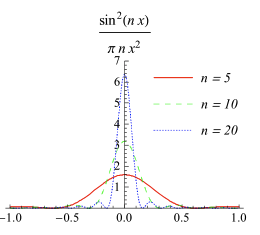
\includegraphics[width=0.9\textwidth,height=2.3in]{figs/5-1.png}
				  \end{center}
			\end{column}
		\end{columns}
\end{frame}

\begin{frame}
	\frametitle{}
	\例 [7. 试证明$\delta$函数的微分公式 ]
	{\[ \delta(x)=\frac{dH(x)}{dx}, \qquad H(x)
		=\left\{\begin{array}{c}
			0, \qquad(x<0) \\
			1, \quad(x >= 0)
			\end{array}\right. \]}
	\证 \[
		\begin{aligned}
		  \int_{-\infty}^{+\infty} \frac{dH(x)}{dx} \psi (x) d x &= H(x) \psi (x)\mid_{-\infty}^{+\infty} - \int_{-\infty}^{+\infty} H(x) \psi' (x) d x \\
		    &=  \psi (+\infty) - \int_{0}^{+\infty} \psi' (x) d x\\
			&=  \psi (+\infty)- \psi (+\infty)+\psi (0)\\
			&=  \psi (0) \\ 
			&=\int_{-\infty}^{+\infty} \delta(x) \psi (x) d x
		\end{aligned}
		   \]
		证毕!
\end{frame}

\begin{frame}
	\frametitle{}
	\例 [8. 试证明$\delta$函数的展开公式]
	{}
	 \[
		\begin{aligned}
		  \delta (\vec{r}-\vec{r}_0) &=  \delta (x-x_0) \delta (y-y_0) \delta (z-z_0)\\
		  &=  \frac{1}{r}\delta (r-r_0) \delta (\theta -\theta_0) \\
		  &=  \frac{1}{r^2\sin\theta}\delta (r-r_0) \delta (\theta -\theta_0) \delta (\varphi -\varphi_0)
		\end{aligned}
		   \]
\end{frame}

%%%%%%%%%%%%%%%%%%%%%%%%%%%%%%%%%%%%%%%%%%%%%%%%%%%%%%%%%%%%%%%%%%%
\begin{frame}
	\frametitle{课堂作业}
	 \begin{exampleblock}{1. 试证明:}
	 \[
	\int_{-\infty}^{+\infty} 1 \cdot e^{2\pi i kx} d x = \delta(k)
	\]
	 \end{exampleblock}
	\begin{exampleblock} {2. 求动量表象波函数}
	{已知坐标表象的波函数如下,现基于$\delta$函数求动量表象的波函数 $c(p)$}
		\begin{equation*}
			\Psi(x)=\frac{1}{\sqrt{2\pi \hbar}}  \int_{-\infty}^{+\infty} c(p) e^{\frac{i}{\hbar} px} dp 
		\end{equation*}   	
	\end{exampleblock}
\begin{exampleblock} {3. 证明第一类贝塞尔函数的正交性公式}
	\[\int_{0}^{+\infty} J_n(kr)J_n(k'r) r dr = \frac{\delta(k-k')}{k}, \qquad (n\geq-1; k, k'>0)\] 
	\end{exampleblock}
\end{frame}
%%%%%%%%%%%%%%%%%%%%%%%%%%%%%%%%%%%%%%%%%%%%%%%%%%%%%%%%%%%%%%%%%%%